%!TEX root = surface_reconstruction.tex
% Добавьте ссылку на файлы с текстом работы
% Можно использовать команды:
%   \input или \include
% Пример:
%    \input{mainfiles/1-section} или \include{mainfiles/2-section}
% Команда \input позволяет включить текст файла без дополнительной обработки
% Команда \include при включении файла добавляет до него и после него команду
% перехода на новую страницу. Кроме того, она позволяет компилировать каждый файл
% в отдельности, что ускоряет сборку проекта.
% ВАЖНО: команда \include не поддерживает включение файлов, в которых уже содержится команда \include,
% т.е. не возможен рекурсивный вызов \include
\newcommand*{\Source}{
    %!TEX root = ../surface_reconstruction.tex
\phantomsection
\section*{Введение} 
\addcontentsline{toc}{section}{Введение}
Проблема определения поверхности по набору точек активно изучается многие годы. Несмотря на распространение методов реконструкции поверхности, многие аспекты проблемы остаются открытыми. Одними из основных трудностей в процессе реконструкции являются сложность формы и шум.  Проекционный оператор MLS [Levin 2003] зарекомендовал себя как мощный метод реконструкции поверхности. 
Метод MLS позволяет достичь простого и эффективного представления.




%Криптосистема Мак-Элиса "--- одна из старейших криптосистем с открытым ключом. Она была предложена в 1978
%Р.~Дж.~Мак-Элисом~\cite{MCEliece}. Данная криптосистема
%основывается на $\mathbf{\mathbb {NP}}$-трудной проблеме в теории
%кодирования. Основная идея её построения  состоит в маскировке
%некоторого кода, имеющего эффективные алгоритмы декодирования, под
%код, не обладающий видимой алгебраической и комбинаторной
%структурой, такие коды принято называть кодами общего положения.
%Эта криптосистема обладает одним важным преимуществом "--- высокой
%скоростью зашифрования и расшифрования. Однако, у неё имеется
%серьёзный недостаток "--- относительно низкая скорость передачи
%($R$). Обычно у кодовых криптосистем $R<1$, тогда как у
%криптосистемы RSA скорость в точности равна $1$.
%
%В этой работе рассматривается обобщение криптосистемы
%Мак-Элиса, предложенное в 1994 коду В.М.
%Сидельниковым~\cite{Sidelnikov1}. В этой работе модификация,
%предложенная В.~М.~Сидельниковым, называется криптосистемой\\
%Мак-Элиса--Сидельникова. Криптосистема Мак-Элиса--Сидельникова
%строится на основе $u$-кратного использования кодов Рида--Маллера
%$RM(r,m)$. Она имеет высокую криптографическую стойкость, скорость
%передачи близкую к $1$ и сравнительно невысокую сложность
%шифрования секретных сообщений и расшифрования криптограмм этих
%сообщений.
%
%В работе исследуются вопросы, связанные с пространством
%эквивалентных секретных ключей, то есть секретных ключей,
%порождающих одинаковые открытые ключи, новой криптосистемы. Опишем
%краткое содержание разделов работы.
%
%В \S~1 даётся определение криптосистемы Мак-Элиса, описываются её
%секретный и открытый ключи. Приводятся алгоритмы зашифрования и
%расшифрования.
%
%В \S~2 изучается ключевое пространство криптосистемы Мак-Элиса.
%Устанавливается связь классов эквивалентностей секретных ключей с
%группой автоморфизмов линейного кода, лежащего в основе этой
%криптосистемы.
%
%В \S~3 описывается криптосистема Мак-Элиса--Сидельникова:
%секретный и открытый ключи, алгоритмы зашифрования и
%расшифрования.
%
%\S~4 посвящён ключевому пространству новой криптосистемы. В нём
%вводятся множества, необходимые для описания классов
%эквивалентности секретных ключей. Получаются нижние и верхние
%оценки на мощности  введённых множеств и на число открытых ключей
%криптосистемы Мак-Элиса--Сидельникова.
%
%В \S~5 изучается криптосистема Мак-Элиса--Сидельникова в случае
%двух блоков ($u=2$).
%
%В настоящей работе получаются нижние оценки на мощность множества
%открытых ключей криптосистемы
%Мак-Элиса--Сидельникова(теорема~\ref{t3}) при использовании
%произвольного числа блоков $u$. Для кодов Рида--Маллера с
%$u$-кратным повторением строится множество, которое, в некотором
%смысле, является аналогом группы автоморфизмов обычного кода
%Рида--Маллера, и устанавливается связь этого множества с классами
%эквивалентности секретных ключей.
%
%Для случая двух блоков ($u=2$) полностью описывается указанное
%множество при использовании кодов Рида--Маллера $RM(r,m)$
%$(r\leqslant 2,r<m)$ и матриц определённого вида
%(теоремы~\ref{theorem1},~\ref{theorem2}). Тем самым при $u=2,
%r\geqslant 2, r<m$ описываются все классы эквивалентности
%секретных ключей с представителями особого вида и вычисляются их
%мощности. Для некоторых классов эквивалентности секретных ключей
%приводятся нижние оценки на их мощность(теоремы~\ref{theorem1}
%и~\ref{theorem2}).

    %!TEX root = ../surface_reconstruction.tex


\section{Описание последовательно алгоритма}
Здесь будет описание последовательного алгоритма  

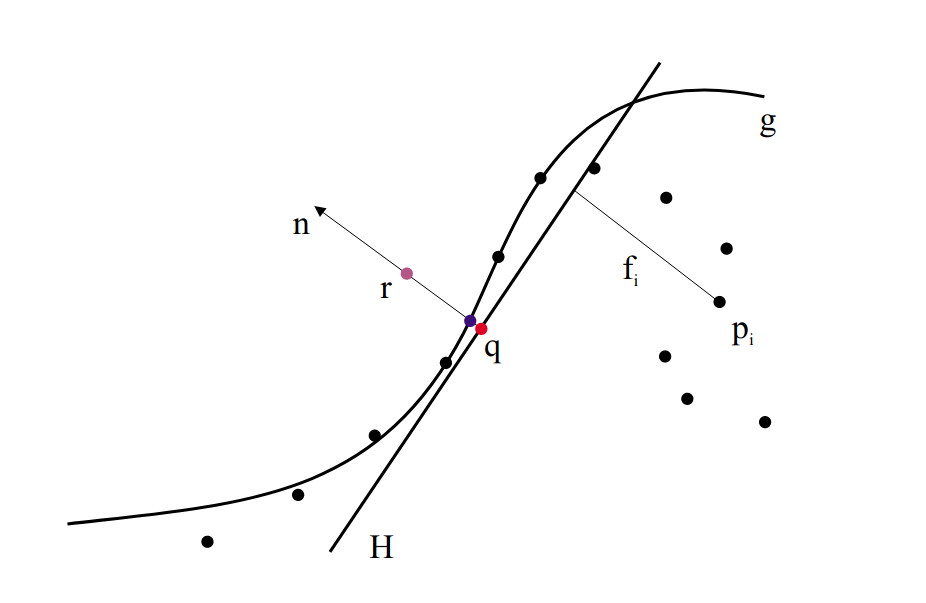
\includegraphics[scale=0.4]{0.png}


\section{Существующие алгоритмы}
\subsection{Оператор локально-оптимальной проекции(LOP)}
Происхождением метода является алгоритм Вайсфельда для решения задачи Ферма-Вебера о расположении точек, также известный как многомерная медиана L1. Это статистический инструмент, который традиционно применяется во всем мире для многомерных непараметрических точечных выборок, чтобы получить хороший представитель для большого количества выборок при наличии шума и выбросов. Проблема была впервые известна как проблема оптимального местоположения Вебера [1909]. Задача состояла в том, чтобы найти оптимальное место для промплощадки, минимизирующее стоимость доступа. В статистике проблема известна как медиана L1 [Brown 1983; Small 1990].

Задача Ферма-Вебера (глобальная) о расположении точек рассматривается как пространственная медиана, поскольку, будучи ограничена одномерным случаем, она совпадает с одномерной медианой и наследует некоторые ее свойства в многомерной постановке.

Реконструкция с помощью оператора проекции имеет важное достоинство: она определяет непротиворечивую геометрию на основе точек данных и предоставляет конструктивные средства для повышения ее дискретизации. 
Оператор локально-оптимальной проекции без параметризации использует более примитивный механизм проецирования, но поскольку он не основан на локальной 2D-параметризации, он более надежен и хорошо работает в сложных сценариях. Кроме того, если точки данных взяты локально с гладкой поверхности, оператор обеспечивает аппроксимацию второго порядка, что приводит к правдоподобной аппроксимации выбранной поверхности.

Оператор LOP имеет две непосредственные функции: во-первых, его можно использовать в качестве этапа предварительной обработки для любого другого метода реконструкции более высокого порядка (например, RBF). LOP можно применять к необработанным отсканированным данным для создания чистого набора данных, в качестве средства эффективного уменьшения шума и выбросов, а также для упрощения определения ориентации и топологии локальной поверхности. Во-вторых, его можно использовать для уточнения данного набора данных.

Для множества точек данных $P = \{p_j\} _j_\in_J \subset \mathbf R^{3}$, LOP проецирует произвольное множество точек $X^{(0)} = \{x_i^{(0)} \} _i_\in_I \subset \mathbf R^{3}$ 


\section{Параллелизм}

Здесь будет параллельный алгоритм на псевдокоде




Параллельный алгоритм

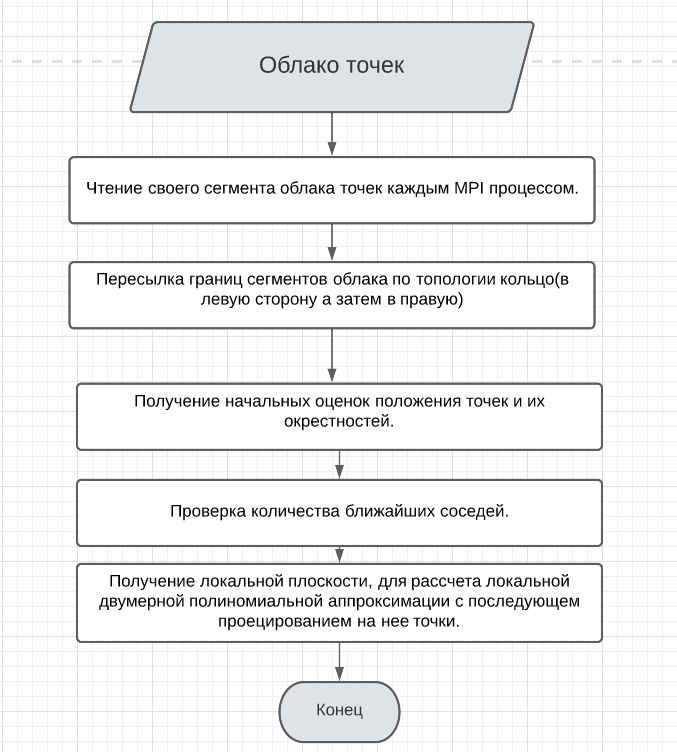
\includegraphics[scale=0.5]{1.png}

\section{Результаты экспериментов}

Время работы на n процессах n = 1...8


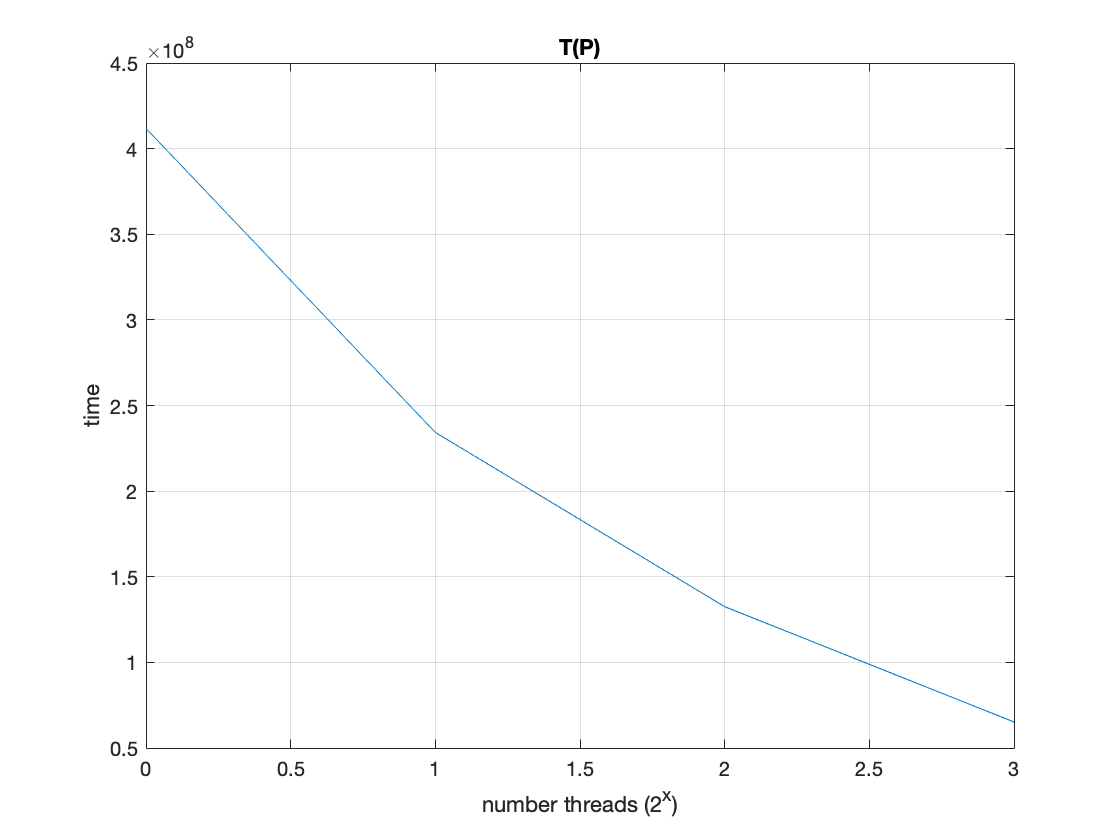
\includegraphics[scale=0.4]{T(P).png}

Ускорение:

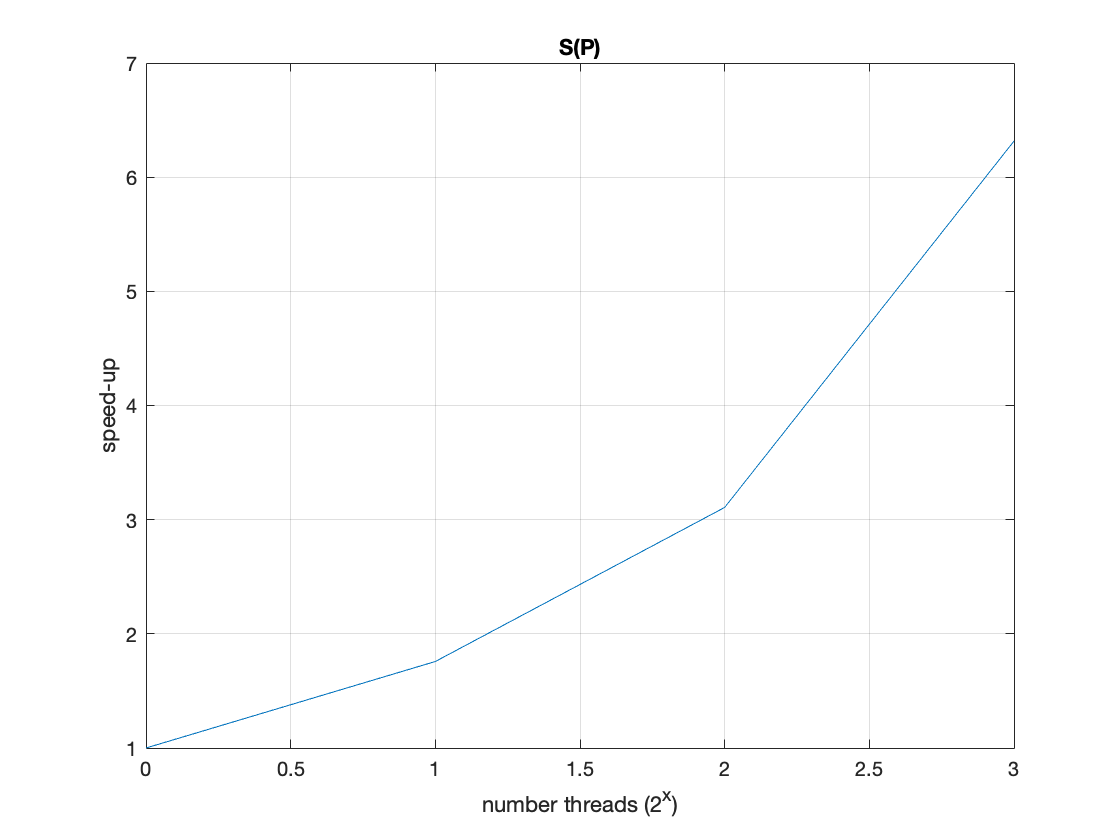
\includegraphics[scale=0.4]{S(P).png}

Эффективность:

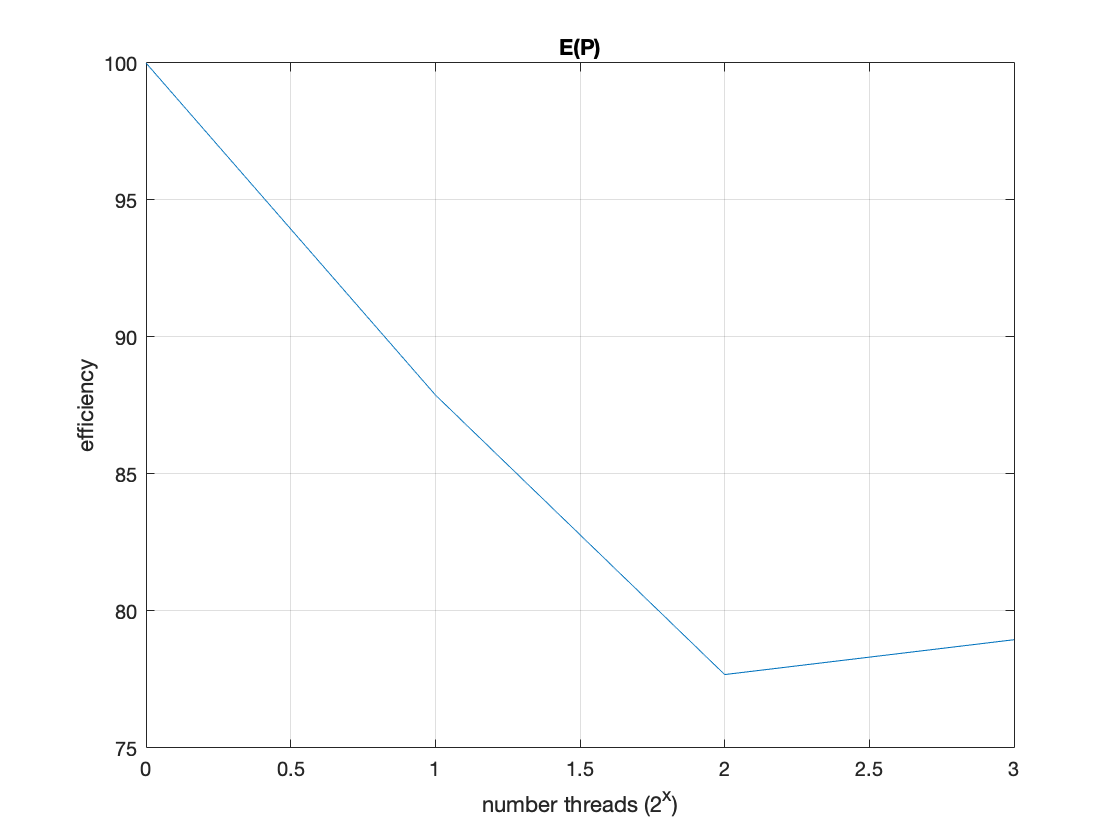
\includegraphics[scale=0.4]{E(P).png}


    %!TEX root = ../surface_reconstruction.tex

\section{Результаты работы}

В работе сформулирован и реализован параллельный алгоритм рекострукции поверхности с использованием программного интерфейса Message Passing Interface для передачи сообщений, завязанный на алгоритме движущихся наименьших квадратов. Алгоритм предусматривает равномерное распределение сегментов облака точек по процессам с последующей пересылкой границ разбиения по топологии кольцо. Все последующие вычисления выполняются локально. Будучи избавленным от последующих пересылок данных, он обеспечивает максимальное ускорение. 
}


% Информация о годе выполнения работы
\def\Year{%
    % 2006%
    \the\year%     % Текущий год
}

% Укажите тип работы
% Например:
%     Выпускная квалификационная работа,
%     Магистерская диссертация,
%     Курсовая работа, реферат и т.п.
\def\WorkType{%
    % Выпускная квалификационная работа%
    % Магистерская диссертация%
    % Курсовая работа%
    % Реферат%
    Курсовая работа%
}

% Название работы
%%%%%%%%%%% ВНИМАНИЕ! %%%%%%%%%%%%%%%%
% В МГУ ОНО ДОЛЖНО В ТОЧНОСТИ
% СООТВЕТСТВОВАТЬ ВЫПИСКЕ ИЗ ПРИКАЗА
% УТОЧНИТЕ НАЗВАНИЕ В УЧЕБНОЙ ЧАСТИ
\def\Title{%
    Реконструкция поверхности методом
    движущихся наименьших квадратов на суперкомпьютере%
}


% Имя автора работы
\def\Author{%
    Хабибулин Марат Ильдарович%
}

% Информация о научном руководителе
%% Фамилия Имя Отчество%
\def\SciAdvisor{%
    Никольский Илья Михайлович%
}
%% В формате: И.~О.~Фамилия%
\def\SciAdvisorShort{%
    И.~М.~Никольский%
}
%% должность научного руководителя
\def\Position{%
    % профессор%
    доцент%
    % старший преподаватель%
    % преподаватель%
    % ассистент%
    % ведущий научный сотрудник%
    % старший научный сотрудник%
    % научный сотрудник%
    % младший научный сотрудник%
}
%% учёная степень научного руководителя
\def\AcademicDegree{%
    % д.ф.-м.н.%
    % д.т.н.%
    к.ф.-м.н.%
    % к.т.н.%
    % без степени%
}

% Информация об организации, в которой выполнена работа
%% Город
\def\Place{%
    Москва%
}
%% Университет
\def\Univer{%
    Московский государственный университет имени М.~В.~Ломоносова%
}
%% Факультет
\def\Faculty{%
    Факультет вычислительной математики и кибернетики%
}
%% Кафедра    
\def\Department{%
    Кафедра информационной безопасности%
}     

%%%% Переключите статус документа для отладки
%%%% В режиме draft документ собирается очень быстро
%%%% и выводится полезная информация о том
%%%% какие строки вылезают за границы документа, что удобно для борьбы с ними
\def\Status{%
    % draft%
    final%
}

%%%% Включает и выключает подпись <<С текстом работы ознакомлен>>
\def\EnableSign{%
     true%
}
